\documentclass[letterpaper]{article} % Each conference has it's own template change the beginning of your main file accordingly
\usepackage[margin=.8in]{geometry}

% The next 6 lines should stay the same for all your projects
%Set to 1 to compile figures, 0 just import pre-generated pdfs 
\def\compileFigures{1}
\newcommand{\filename}{main}
\newcounter{figureNumber}
% !TeX root = main.tex
\PassOptionsToPackage{svgnames}{xcolor}
\usepackage{graphicx}
\usepackage{hyperref}
\usepackage{amsmath}
\usepackage{booktabs}

\usepackage{tikz}
\if\compileFigures1
\usetikzlibrary{external}
\tikzexternalize[prefix=fig/] % activate!
\fi

\usepackage{pgfplots}
\usetikzlibrary{shadings,shadows}

\usepgfplotslibrary{fillbetween}
\usetikzlibrary{patterns}
\usetikzlibrary{positioning}



%Pgfplot commands
\pgfplotsset{
	box plot/.style={
		/pgfplots/.cd,
		only marks,
		mark=-,
		mark size=1em,
		/pgfplots/error bars/.cd,
		y dir=plus,
		y explicit,
	},
	box plot box/.style={
		/pgfplots/error bars/draw error bar/.code 2 args={%
			\draw  ##1 -- ++(1em,0pt) |- ##2 -- ++(-1em,0pt) |- ##1 -- cycle;
		},
		/pgfplots/table/.cd,
		y index=2,
		y error expr={\thisrowno{3}-\thisrowno{2}},
		/pgfplots/box plot
	},
	box plot top whisker/.style={
		/pgfplots/error bars/draw error bar/.code 2 args={%
			\pgfkeysgetvalue{/pgfplots/error bars/error mark}%
			{\pgfplotserrorbarsmark}%
			\pgfkeysgetvalue{/pgfplots/error bars/error mark options}%
			{\pgfplotserrorbarsmarkopts}%
			\path ##1 -- ##2;
		},
		/pgfplots/table/.cd,
		y index=4,
		y error expr={\thisrowno{2}-\thisrowno{4}},
		/pgfplots/box plot
	},
	box plot bottom whisker/.style={
		/pgfplots/error bars/draw error bar/.code 2 args={%
			\pgfkeysgetvalue{/pgfplots/error bars/error mark}%
			{\pgfplotserrorbarsmark}%
			\pgfkeysgetvalue{/pgfplots/error bars/error mark options}%
			{\pgfplotserrorbarsmarkopts}%
			\path ##1 -- ##2;
		},
		/pgfplots/table/.cd,
		y index=5,
		y error expr={\thisrowno{3}-\thisrowno{5}},
		/pgfplots/box plot
	},
	box plot median/.style={
		/pgfplots/box plot
	}
}
% !TeX root = main.tex
\newcommand{\R}[0]{\mathbb{R}}
\newcommand{\E}[0]{\mathbb{E}}

\DeclareMathOperator*{\argmax}{arg\,max}
\DeclareMathOperator*{\argmin}{arg\,min}

%Colormaps
\pgfplotsset{
	colormap={mygreen}{rgb255(0cm)=(254,254,254);rgb255(1cm)= (4,101,53)},
	colormap={myblue}{rgb255(0cm)=(160,30,50); rgb255(1cm)=(39,59,129)},
	colormap={myred}{rgb255(0cm)=(254,254,254); rgb255(1cm)=(160,30,50)},
	colormap={mybred}{rgb255(0cm)=(254,254,254); rgb255(1cm)=(217,10,100)},
	colormap={mybblue}{rgb255(0cm)=(217,10,100); rgb255(1cm)=(10,157,217)},
	colormap={mybgreen}{rgb255(0cm)=(254,254,254); rgb255(1cm)=(98,159,67)}
}

\definecolor{blue}{RGB}{31,120,180}
\definecolor{bblue}{RGB}{166,206,227}
\definecolor{green}{RGB}{ 251,154,153}
\definecolor{red}{RGB}{51,160,44}
\definecolor{bred}{RGB}{178,223,138} 


\title{Project template}

\begin{document}
\maketitle	

% !TeX root = ../main.tex
\section{Figures}\label{sec:figures}
There are two wonderful packages in LaTeX to create figures TikZ and PGFPlots. The former can be used to create any kind of vector graphic, the latter focuses on plots. Together they can create almost any kind of figure you need for a paper. Use them. Here, some examples from a recent paper \cite{ganesh2023impact}: 

\begin{figure*}[hbtp]
	\centering
	\addtolength{\tabcolsep}{-8pt}
	\begin{tabular}{cc}
		\textbf{(a) Fairness} & \textbf{(b) Performance} \\[0.2cm]
	    \if\compileFigures1
			% !TeX root = ../main.tex
\begin{tikzpicture}[rotate=-90,transform shape]
	\begin{axis}[title={}, width=0.3\linewidth,height=0.65\linewidth, ymin=0,ymax=10,yticklabel= {\color{red} \pgfmathprintnumber\tick\%}, ylabel={\small \color{red} Average Odds},ylabel near ticks, yticklabel pos=right, enlarge x limits=0.25, x tick label style={font=\small}, y tick label style={font=\small}, xticklabels={Baseline, Reweighing, EO Loss, FairBatch}, xtick={0,1,2,3},xmin=0,xmax=3,xticklabel style={rotate=90, anchor=east},yticklabel style={rotate=90, anchor=north}]
		\addplot [red,box plot median] table {data/acsincome/variance_introduction_mitigation_avgodds.dat};
		\addplot [red,box plot box] table {data/acsincome/variance_introduction_mitigation_avgodds.dat};
		\addplot [red,box plot top whisker] table {data/acsincome/variance_introduction_mitigation_avgodds.dat};
		\addplot [red,box plot bottom whisker] table {data/acsincome/variance_introduction_mitigation_avgodds.dat};
	\end{axis}
\end{tikzpicture}
		\else
			\includegraphics[]{fig/\filename-figure\thefigureNumber.pdf}
			\stepcounter{figureNumber}
		\fi
	 &  \if\compileFigures1
			\begin{tikzpicture}[rotate=-90,transform shape]
	\begin{axis}[title={}, scale=0.8, width=0.32\linewidth,height=0.35\linewidth, ymin=78,ymax=82,yticklabel= {\color{blue} \pgfmathprintnumber\tick\%}, ylabel={\small \color{blue} $F_1$ Score{\color{white}y}},ylabel near ticks, yticklabel pos=right, enlarge x limits=0.25, x tick label style={font=\small}, y tick label style={font=\small}, xticklabels={}, ytick={78,79,80,81,82}, xtick={0,1,2,3},xmin=0,xmax=3,xticklabel style={rotate=90, anchor=east},yticklabel style={rotate=90, anchor=north}]
		\addplot [blue,box plot median] table {data/acsincome/variance_introduction_mitigation_fscore.dat};
		\addplot [blue,box plot box] table {data/acsincome/variance_introduction_mitigation_fscore.dat};
		\addplot [blue,box plot top whisker] table {data/acsincome/variance_introduction_mitigation_fscore.dat};
		\addplot [blue,box plot bottom whisker] table {data/acsincome/variance_introduction_mitigation_fscore.dat};
	\end{axis}
\end{tikzpicture}
		\else
			\includegraphics[]{fig/\filename-figure\thefigureNumber.pdf}
			\stepcounter{figureNumber}
		\fi \\
	\end{tabular}
	\caption{ Some box plots}
	\label{fig:variance_introduction}
\end{figure*}


\begin{figure*}[hbtp]
	\centering
	\if\compileFigures1
		% !TeX root = ../main.tex
\begin{tikzpicture}[scale=1.2, 
	mynode/.style = {rectangle, align=center,font={\tiny}},
	myalertnode/.style = {rectangle, align=left,font={\tiny},text=mLightBrown},   -stealth
	]
	\node (data) at (-3,0) {
\includegraphics[height=40px]{images/data.png}};
	\node[above = -0.1cm of data] (datatitle) {Dataset}; 
	
	\node (trainingset) at (0,1) {
\includegraphics[height=30px]{images/data.png}};
	\node[above = -0.1cm of trainingset] (trainingtitle) {Training data};
	
	\node (testset) at (0,-1) {
\includegraphics[height=30px]{images/data.png}};
	\node[below = -0.1cm of testset] (testtitle) {Test data};
	
	\node (initmodel) at (-3,3) {
\includegraphics[height=40px]{images/noun-blueprint.png}};
	\node[above = -0.1cm of initmodel] (modeltitle) {Model architecture}; 
	
	\node (currentmodel) at (3,3) {
\includegraphics[height=30px]{images/model.png}};
	\node[above = -0.1cm of currentmodel] (currentmodeltitle) {Current Model}; 
	
	\node (shuffle) at (3,1) {
\includegraphics[height=30px]{images/data.png}};
	\node[above = -0.1cm of shuffle] (shuffletitle) {Shuffled data}; 
	
	\node (training) at (6,2) {
\includegraphics[height=40px]{images/noun_data_processing.png}};
	
	\node (Training loop) at (6,4) {\Large{\textbf{Training loop}}}; 
	
	\node (trainedmodel) at (9,2) {
\includegraphics[height=30px]{images/model.png}};
	\node[above = -0.1cm of trainedmodel] (modeloutputtitle) {Final  Model}; 
	
	\node (evaluation) at (9,-1) {
\includegraphics[height=30px]{images/noun_evaluate.png}};
	\node[below = -0.1cm of evaluation] (evaluationtitle) {Evaluation}; 
	
	\node[right = 0.4cm of data]  (splitting) {\colorbox{blue!20}{\color{blue} \textbf{(a) Data splitting}}};
	
	\draw[rounded corners](1.5,0.2)--(7.5,0.2)--(7.5,4.3)--(1.5,4.3)--cycle;
	
	\draw[-stealth,ultra thick] (data.east) -- (trainingset.west);
	\draw[-stealth,ultra thick] (data.east) -- (testset.west);
	
	\draw[-stealth,ultra thick] (trainingset.east) -- (shuffle.west);
	\draw[-stealth,ultra thick] (initmodel.east) -- node[above] {\colorbox{blue!20}{\color{blue} \textbf{(b) Initialization }}} (currentmodel.west);
	
	\draw[-stealth,ultra thick] (training.east) -- (trainedmodel.west);
	
	\draw[-stealth,ultra thick] (testset.east) -- (evaluation.west);
	\draw[-stealth,ultra thick] (trainedmodel.south) -- (evaluation.north);
	
	
	\begin{scope}[transform canvas={yshift=.7em}]
		\path[-stealth,ultra thick, shorten <=2mm, shorten >=2mm] (currentmodel.east) edge[bend left] (training.west);
		\path[-stealth,ultra thick, shorten <=2mm, shorten >=2mm] (training.west)  edge[bend left] (currentmodel.east) ;
	\end{scope}
	
	\path[-stealth,ultra thick, shorten <=2mm, shorten >=2mm] (shuffle.east) edge[bend left] (training.west);
	\path[-stealth,ultra thick, shorten <=2mm, shorten >=2mm] (training.west)  edge[bend left] node[below right] {\colorbox{blue!20}{\color{blue} \textbf{(c) (Re)shuffling}}} (shuffle.east) ;
	
	
	\draw[-stealth,ultra thick] (testset) -- (evaluation.west);
	
\end{tikzpicture} 
	\else
		\includegraphics[]{fig/\filename-figure\thefigureNumber.pdf}
	\stepcounter{figureNumber}
	\fi 
	\caption{An overview}
	\label{fig:overview}
\end{figure*}


\begin{figure*}[htbp]
	\centering
	\if\compileFigures1
		% !TeX root = ../main.tex
\begin{tikzpicture}[]
	\begin{axis}[scale=0.7,title={\textbf{(a) Normal training}}, width=0.32\linewidth,height=0.28\linewidth, ymin=79,ymax=79.9,yticklabel= {\pgfmathprintnumber\tick\%}, ylabel={\small $F_1$ Score},ylabel near ticks, enlarge x limits=0.2, xticklabel= {\pgfmathprintnumber\tick\%}, xlabel={\small Average Odds}, x tick label style={font=\small,text width=1cm,xshift=0.35cm}, y tick label style={font=\small}, xmin=5.8,xmax=9.2,xtick={6,7,8,9},legend pos=south east,legend cell align=left,legend style={draw=none,font=\scriptsize},axis background/.style={}]
		\addplot[green,only marks,mark size=1.2pt] table[x index=0, y index=1] {data/acsincome/decouple_scatter_all.dat};
	\end{axis}
\end{tikzpicture}%
$\qquad$
\begin{tikzpicture}[]
	\begin{axis}[scale=0.7,title={\textbf{(b) Fixed Reshuffling}}, width=0.32\linewidth,height=0.28\linewidth, ymin=79,ymax=79.9,ymajorticks=false,ylabel near ticks, enlarge x limits=0.2, xticklabel= {\pgfmathprintnumber\tick\%}, xlabel={\small Average Odds}, x tick label style={font=\small,text width=1cm,xshift=0.35cm}, y tick label style={font=\small}, xmin=5.8,xmax=9.2,xtick={6,7,8,9},legend pos=south east,legend cell align=left,legend style={draw=none,font=\scriptsize},axis background/.style={}]
		\addplot[blue,only marks,mark size=1.2pt] table[x index=0, y index=1] {data/acsincome/decouple_scatter_weight.dat};
	\end{axis}
\end{tikzpicture}%
$\qquad$
\begin{tikzpicture}[]
	\begin{axis}[scale=0.7,title={\textbf{(c) Fixed Weight Init}}, width=0.32\linewidth,height=0.28\linewidth, ymin=79,ymax=79.9,ymajorticks=false,ylabel near ticks, enlarge x limits=0.2, xticklabel= {\pgfmathprintnumber\tick\%}, xlabel={\small Average Odds}, x tick label style={font=\small,text width=1cm,xshift=0.35cm}, y tick label style={font=\small}, xmin=5.8,xmax=9.2,xtick={6,7,8,9},legend pos=south east,legend cell align=left,legend style={draw=none,font=\scriptsize},axis background/.style={}]
		\addplot[red,only marks,mark size=1.2pt] table[x index=0, y index=1] {data/acsincome/decouple_scatter_shuffle.dat};
	\end{axis}
\end{tikzpicture}

	\else
		% The file contains three figures so wee need to include three here
		\includegraphics[]{fig/\filename-figure\thefigureNumber.pdf}
		\stepcounter{figureNumber}
		\includegraphics[]{fig/\filename-figure\thefigureNumber.pdf}
		\stepcounter{figureNumber}
		\includegraphics[]{fig/\filename-figure\thefigureNumber.pdf}
		\stepcounter{figureNumber}
	\fi 	
	\caption{Some scatterplots}
	\label{fig:decouple_scatter}
\end{figure*}


\begin{figure*}[htbp]
	\centering	
	\if\compileFigures1
		% !TeX root = ../main.tex
\begin{tikzpicture}
	\begin{axis} [scale=0.8, width=0.4\linewidth,height=0.28\linewidth,yticklabel= {\pgfmathprintnumber\tick\%}, ylabel={Average Odds},ymin=5.5,ymax=10.5,xmin=100,xmax=300,xlabel=Epoch,axis y line*=left,axis x line*=bottom,ylabel near ticks,title= {\textbf{(a) Fixed Data Reshuffling}},legend style={at={(1.02,1.05)},draw=none,font=\scriptsize,empty legend}]
		
		\addplot [blue,no marks, thick] table[x=x,y=y1] {data/acsincome/curve_correlation_weight.dat};
		\addplot [name path=topw,opacity=0.,no marks] table[x=x,y=y2] {data/acsincome/curve_correlation_weight.dat};
		\addplot [name path=botw,opacity=0.,no marks] table[x=x,y=y3] {data/acsincome/curve_correlation_weight.dat};
		\addplot[blue,opacity=0.5] fill between[of=topw and botw];
		\addplot [name path=topwm,opacity=0.,no marks] table[x=x,y=y4] {data/acsincome/curve_correlation_weight.dat};
		\addplot [name path=botwm,opacity=0.,no marks] table[x=x,y=y5] {data/acsincome/curve_correlation_weight.dat};
		\addplot[blue,opacity=0.2] fill between[of=topwm and botwm];
		
	\end{axis}
\end{tikzpicture}
\begin{tikzpicture}
	\begin{axis} [scale=0.8, width=0.4\linewidth,height=0.28\linewidth,yticklabel= {\pgfmathprintnumber\tick\%},ymin=5.5,ymax=10.5,xmin=100,xmax=300,xlabel=Epoch,axis y line*=left,axis x line*=bottom,ylabel near ticks,title= {\textbf{(b) Fixed Weight Initialization}},legend style={at={(1.02,1.05)},draw=none,font=\scriptsize,empty legend},ymajorticks=false]
		
		\addplot [red,no marks, thick] table[x=x,y=y1] {data/acsincome/curve_correlation_shuffle.dat};
		\addplot [name path=tops,opacity=0.,no marks, thick] table[x=x,y=y2] {data/acsincome/curve_correlation_shuffle.dat};
		\addplot [name path=bots,opacity=0.,no marks, thick] table[x=x,y=y3] {data/acsincome/curve_correlation_shuffle.dat};
		\addplot[red,opacity=0.5] fill between[of=tops and bots];
		\addplot [name path=topsm,opacity=0.,no marks, thick] table[x=x,y=y4] {data/acsincome/curve_correlation_shuffle.dat};
		\addplot [name path=botsm,opacity=0.,no marks, thick] table[x=x,y=y5] {data/acsincome/curve_correlation_shuffle.dat};
		\addplot[red,opacity=0.2] fill between[of=topsm and botsm];
		
	\end{axis}
\end{tikzpicture}
		\raisebox{1.03cm}{
		% !TeX root = ../main.tex
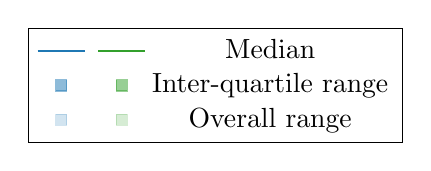
\begin{tikzpicture}
	\begin{axis}[scale=0.01,
		hide axis,
		xmin=0, xmax=1,
		ymin=0, ymax=1,
		legend columns=2,
		%legend style={draw=none}
		]
		\addlegendimage{blue,thick}
		\addlegendentry{};
		\addlegendimage{red,thick}
		\addlegendentry{Median};
		\addlegendimage{blue,opacity=0.5,mark=square*, only marks}
		\addlegendentry{};
		\addlegendimage{red,opacity=0.5,mark=square*, only marks}
		\addlegendentry{Inter-quartile range};
		\addlegendimage{blue,,opacity=0.2,mark=square*, only marks}
		\addlegendentry{};
		\addlegendimage{red,,opacity=0.2,mark=square*, only marks}
		\addlegendentry{Overall range};
	\end{axis}
\end{tikzpicture}

		}
	\else
		% The files contain three figures so wee need to include three here
		\includegraphics[]{fig/\filename-figure\thefigureNumber.pdf}
		\stepcounter{figureNumber}
		\includegraphics[]{fig/\filename-figure\thefigureNumber.pdf}
		\stepcounter{figureNumber}
		\raisebox{1.03cm}{
		\includegraphics[]{fig/\filename-figure\thefigureNumber.pdf}
		}
		\stepcounter{figureNumber}
	\fi 
	\caption{And some line plots with a legend}
	\label{fig:decouple_correlation}
\end{figure*}

\section{Tables}\label{sec:tables}

Use the booktabs package. Ideally only have three horizontal lines. Don't have vertical lines! Generally follow the advise \href{https://people.inf.ethz.ch/markusp/teaching/guides/guide-tables.pdf}{here}.


\begin{table*}
	\begin{center}
		\caption{Some tables}
		\label{tab:correlation_others}
		\begin{minipage}{0.48\textwidth}
			\centering
			\textbf{(a) Different Datasets}\\[0.2cm]
			\begin{tabular}{lcc}
				\toprule
				& Fixed RR & Fixed WI \\
				\midrule
				ACSIncome & .94 & .04 \\
				ACSEmployment {\color{white}aa} & .89 & .01 \\
				CelebA & .92 & .01 \\
				\bottomrule
			\end{tabular} \\ [0.2cm]
			\textbf{(b) Different Fairness Metrics}\\[0.2cm]
			\begin{tabular}{lcc}
				\toprule
				& Fixed RR & Fixed WI \\
				\midrule
				Average Odds & .94 & .04 \\
				Equal Opportunity & .94 & .05 \\
				Demographic Parity & .96 & .03 \\
				\bottomrule
			\end{tabular} \\
		\end{minipage}\hfill
		\begin{minipage}{0.48\textwidth}
			\centering
			\textbf{(c) Changing Hyperparameters}\\[0.2cm]
			\begin{tabular}{lcc}
				\toprule
				& Fixed RR & Fixed WI \\
				\midrule
				Default Hyperparameters & .94 & .04 \\
				Batch Size = 16 & .95 & .00 \\
				Learning Rate = 0.01 & .93 & .00 \\
				Arch = \{2048, 64\} & .92 & .00 \\
				\addlinespace[2ex]
				No Dropout & .94 & .04 \\
				Dropout Rate = 10\% & .88 & .03 \\
				Dropout Rate = 20\% & .85 & .04 \\
				Dropout Rate = 30\% & .80 & .13 \\
				\bottomrule
			\end{tabular} \\ [0.2cm]
		\end{minipage}\hfill
	\end{center}
\end{table*}

	
%Bibliography
\bibliographystyle{abbrv}
\bibliography{references}

\end{document}